\section{Analytical Methods}
\label{sec:foundations:methods}

The proposed system applies several analytical and statistical methods
beyond the visualisation primitives and the warehouse architecture.
Algorithmic parameters and implementation details are left to the
per-chart Methodology Side-Panel of
Section~\ref{sec:solution:viz:methodology}.

\noindent\textbf{MoSCoW Prioritisation.}
The MoSCoW scheme partitions candidate requirements into four tiers:
Must have, Should have, Could have, and Won't have (this time).
Section~\ref{sec:solution:problem:questions} uses the scheme to tag
each of the fourteen stakeholder questions with a priority.

\noindent\textbf{Pareto Principle and Heavy-Tailed Distributions.}
The Pareto principle (roughly 20\% of entities account for 80\% of
volume) is a useful diagnostic for choosing top-$k$ ranked bars over
distribution plots. The boarding distribution across routes in the
present project is heavy-tailed, which motivates the ranked-bar
choice in the Demand and Crowding theme.

\subsection{Forecasting}
\label{sec:foundations:methods:prophet}

Error, Trend, Seasonality (ETS) is an exponential smoothing framework
that models a time series as the composition of three state components:
an error term (additive or multiplicative), a trend component (none,
additive, or damped), and a seasonal component (none, additive, or
multiplicative). The \texttt{statsforecast} library
\cite{statsforecast} implements model selection over the full ETS
family (\texttt{AutoETS}), choosing the best-fitting variant by the
Akaike Information Criterion on the training window. The model outputs
point forecasts together with prediction intervals derived from the
fitted component variances. The proposed system uses
\texttt{statsforecast}'s \texttt{AutoETS} model for the fourteen-day
per-route demand forecast of requirement R15. The weekly and yearly
seasonal components capture the commuter-weekday and T\^et-holiday
cycles inherent in bus demand without requiring explicit holiday
regressors.

\subsection{Causal Analysis}
\label{sec:foundations:methods:did}

Difference-in-differences (DiD) is a causal-inference technique that
estimates the effect of a treatment (in this project, a promotion
applied to a subset of routes) by comparing the change in outcome
before and after the treatment between the treated routes and a
control group, where the control group is chosen so that its
pre-treatment trend parallels that of the treated routes. The
estimator is the \emph{difference} between the two
\emph{differences} (post-minus-pre on the treated side, post-minus-pre
on the control side); it cancels common trends and isolates the
treatment effect under the parallel-trends assumption.

When no clean control group exists in the data, a matched comparison
set is constructed from untreated entities whose pre-treatment
trajectory resembles the treated entity. The proposed system uses a
$k$-nearest-neighbour matched-control heuristic in the UMAP archetype
space of Section~\ref{sec:solution:viz:routes}: each treated route is
matched against its $k=5$ nearest neighbours of the same archetype,
and the average of their pre-and-post trajectories serves as the
counterfactual. This heuristic adapts the matched-comparison idea to
the UMAP embedding; it does not implement Abadie's convex-weighted
synthetic-control estimator \cite{abadie2005did}, which optimises
donor weights on the pre-treatment trajectory to satisfy a
parallel-trends criterion that is not verified here.
Figure~\ref{fig:foundations:did} illustrates the construction.

\begin{figure}[!htbp]
\centering
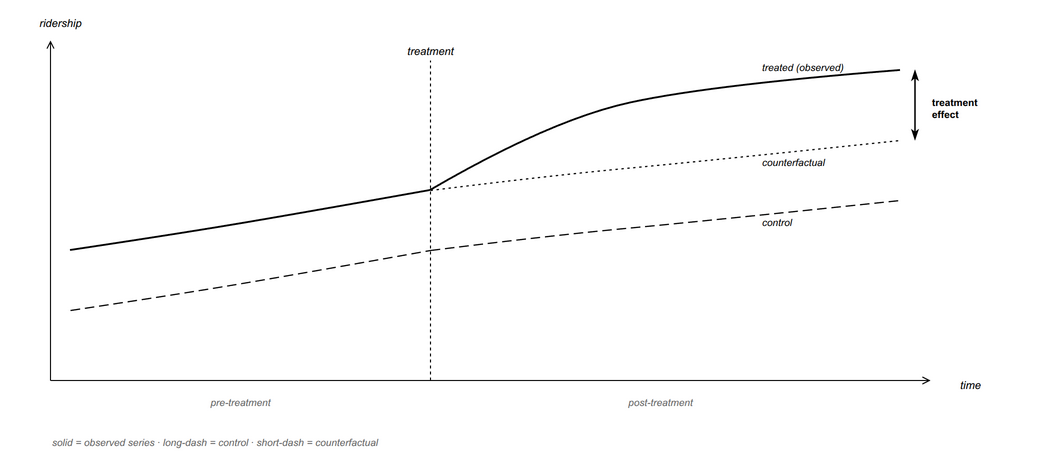
\includegraphics[width=0.92\linewidth]{images/diagrams/foundations_did.png}
\caption{Difference-in-differences with a synthetic control.}
\label{fig:foundations:did}
\end{figure}

\subsection{Concentration Index}
\label{sec:foundations:methods:hhi}

The Herfindahl-Hirschman Index (HHI) summarises market concentration
as the sum of squared market shares across firms
\cite{rhoades1993herfindahl}. For $n$ firms with shares $s_1, s_2,
\dots, s_n$ (each $s_i$ between 0 and 1), the index is

\[
\mathrm{HHI} \;=\; \sum_{i=1}^{n} s_i^2.
\]

The index ranges from $1/n$ (perfect symmetry across $n$ firms) to
$1$ (single-firm monopoly). The proposed system reports HHI at the
network level and per corridor in the Financial and Operations theme
of Section~\ref{sec:solution:viz:financial} as the analytical anchor
for the market-structure treemap; thresholds for concentration alerts
are configured by the analyst on the Methodology Side-Panel.

\subsection{Latency}
\label{sec:foundations:methods:nielsen}

Three established response-time limits from the human-computer
interaction literature are 0.1 seconds for the system to feel
\emph{instantaneous}, 1.0 second for the user's flow of thought to
remain uninterrupted, and 10 seconds for the user's attention to be
retained on the task~\cite{nielsen1993usability}. The proposed
system's non-functional requirement N1 of
Section~\ref{sec:solution:problem:nonfunctional} carries the
0.1-second threshold as its perceived-instantaneous budget and
tightens it to 0.05 seconds for cross-chart brushing under Multiple
Coordinated Views, because the brushing transition must complete
within the human-perception envelope while leaving headroom for the
browser repaint.
